\documentclass[aspectratio=141,10pt]{beamer}

% Look of the lecture slides: white, dark red titles, grey text
\usepackage[T1]{fontenc}
\usepackage[scaled=0.92]{helvet}
\renewcommand{\familydefault}{\sfdefault}
\usepackage{amsmath,amssymb}
\usepackage{booktabs,colortbl,array}
\usepackage{graphicx}

\definecolor{aimsred}{HTML}{990000}
\definecolor{rowpink}{HTML}{F7E9E9}
\definecolor{textgrey}{HTML}{404040}

\usetheme{default}
\setbeamertemplate{navigation symbols}{}
\setbeamercolor{normal text}{fg=textgrey,bg=white}
\setbeamercolor{structure}{fg=aimsred}
\setbeamerfont{frametitle}{series=\bfseries,size=\Large}
\setbeamertemplate{frametitle}{\vskip1.0em\centering\usebeamerfont{frametitle}\color{aimsred}\insertframetitle\par\vskip0.3em}
\setbeamertemplate{itemize item}{\color{aimsred}$\bullet$}
\setbeamertemplate{footline}{\hfill\color{textgrey}\footnotesize\insertframenumber\hspace{1em}\vspace{0.6em}}

\newcommand{\callout}[2]{%
  \begin{center}\fcolorbox{aimsred}{rowpink!60}{\begin{minipage}{#1}\centering #2\end{minipage}}\end{center}}
\newcommand{\hl}[1]{{\bfseries\color{aimsred}#1}}

\begin{document}

% ---------------- Title ----------------
\begin{frame}[plain]
\centering
\vspace{0.5em}

\includegraphics[height=2.4cm]{img/logo1.png}\\[1.6em]
{\Large\color{textgrey} Training Workshop on Mathematical Biology 2026}\\[1.2em]
{\Large\bfseries\color{aimsred} Does the disease survive?\\[0.3em]
Stochastic versus deterministic models of\\ endemic and multi-strain infections}\\[0.8em]
{\normalsize\color{textgrey} Project 3}\\[1.6em]

\includegraphics[height=1.3cm]{img/logo2.png}\hspace{1.5cm}

\includegraphics[height=1.0cm]{img/logo3.png}\hspace{1.5cm}

\includegraphics[height=0.9cm]{img/logo0.png}
\end{frame}

% ---------------- 1. Problem ----------------
\begin{frame}{Will an infection survive? Two models can disagree}
\begin{itemize}\setlength\itemsep{0.9em}
  \item An infection spreads, people recover, and their \hl{immunity wears off}, so they can be infected again.
  \item Two questions:
  \begin{itemize}\setlength\itemsep{0.4em}
    \item does the infection stay in the population for good (\hl{endemic}), or disappear?
    \item when \hl{two strains} compete, do both survive?
  \end{itemize}
  \item Two standard models answer them: a \hl{deterministic} model (ODE) and a \hl{stochastic} model that follows individual people.
  \item \textbf{Our question: when do the two models give the same answer, and when not?}
\end{itemize}
\callout{0.88\textwidth}{\textbf{Why it matters:} whether a disease persists in a community, or a strain can disappear, depends on which model we trust.}
\end{frame}

% ---------------- 2. Approach ----------------
\begin{frame}{Approach: the same events, followed in two ways}
\centering
\renewcommand{\arraystretch}{1.5}
\begin{tabular}{l l l}
\rowcolor{aimsred}\color{white}& \color{white}ODE (deterministic) & \color{white}Gillespie SSA (stochastic)\\
Number infected & a continuous number & a whole number of people\\
\rowcolor{rowpink} Result & one smooth curve & a random path, different each run\\
Can reach zero? & never & yes, and then it is \hl{final}\\
\end{tabular}
\\[1.2em]
\begin{itemize}\setlength\itemsep{0.6em}
  \item Events: infection, recovery, loss of immunity (and births and deaths in the two strain model). Each has a rate.
  \item SSA: wait a random time, pick one event at random according to the rates, update the counts, repeat.
  \item We run the SSA hundreds of times and compare the outcomes with the ODE.
\end{itemize}
\callout{0.8\textwidth}{In the SSA, once nobody is infected, nobody can be infected again.}
\end{frame}

% ---------------- 3. Part 1 model ----------------
\begin{frame}{One strain: the ODE predicts persistence when $N>15$}
\centering
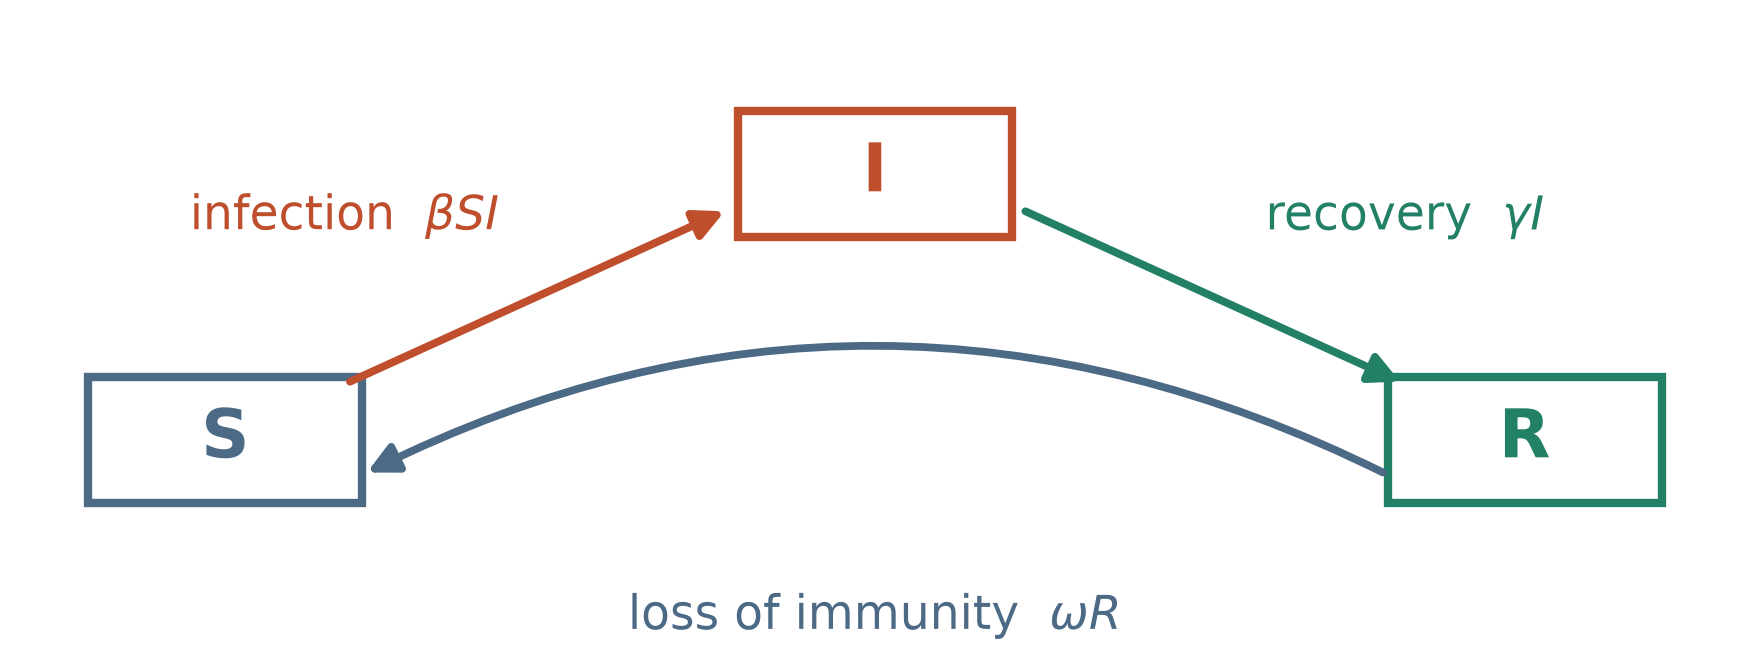
\includegraphics[width=0.66\textwidth]{img/slide_p1_cartoon.png}\\[0.3em]
\callout{0.92\textwidth}{The ODE has an endemic level exactly when the population size is $N>N_c=\dfrac{\gamma}{\beta}=15$:\quad
$I^*=\dfrac{\omega}{\omega+\gamma}\Big(N-\dfrac{\gamma}{\beta}\Big)$}
{\small Infection $\beta=0.01$, recovery $\gamma=0.15$ (about 7 days), loss of immunity $\omega=0.025$ (about 40 days), per day. One infected person at the start.}
\end{frame}

% ---------------- 4. Part 1 result ----------------
\begin{frame}{Above this threshold, small populations still lose the infection}
\centering
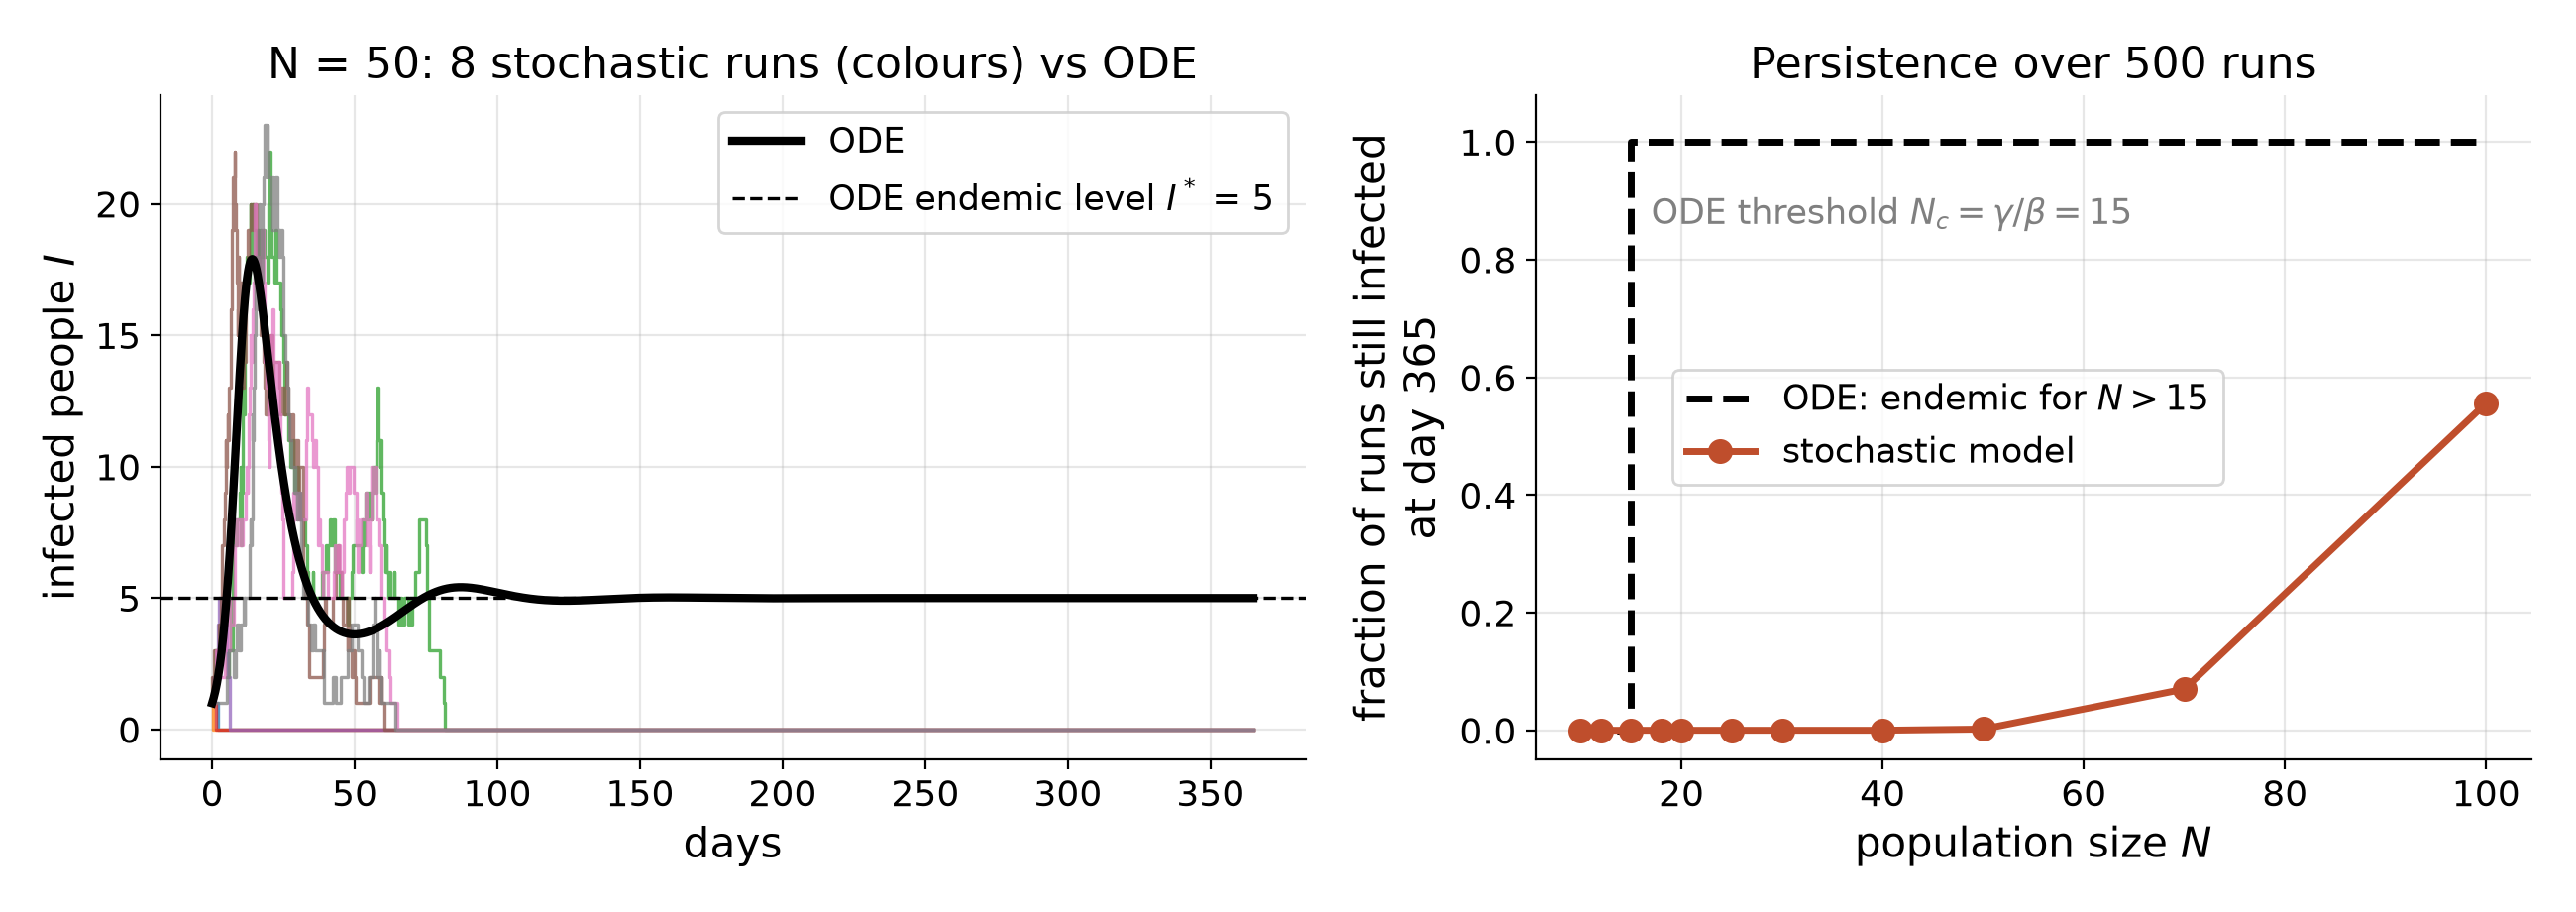
\includegraphics[width=\textwidth]{img/slide_p1_persistence.png}
\begin{itemize}\setlength\itemsep{0.4em}
  \item At $N=50$ the ODE settles at 5 infected people. All 8 stochastic runs reach zero within 3 months.
  \item Out of 500 runs, \hl{none} is still infected after one year up to $N=40$, 7\% at $N=70$, 56\% at $N=100$.
  \item When the infection does survive, its mean level matches the ODE (12.0 against 12.1 people at $N=100$).
\end{itemize}
\end{frame}

% ---------------- 5. Part 2 model ----------------
\begin{frame}{Two strains: immunity to one does not protect from the other}
\centering
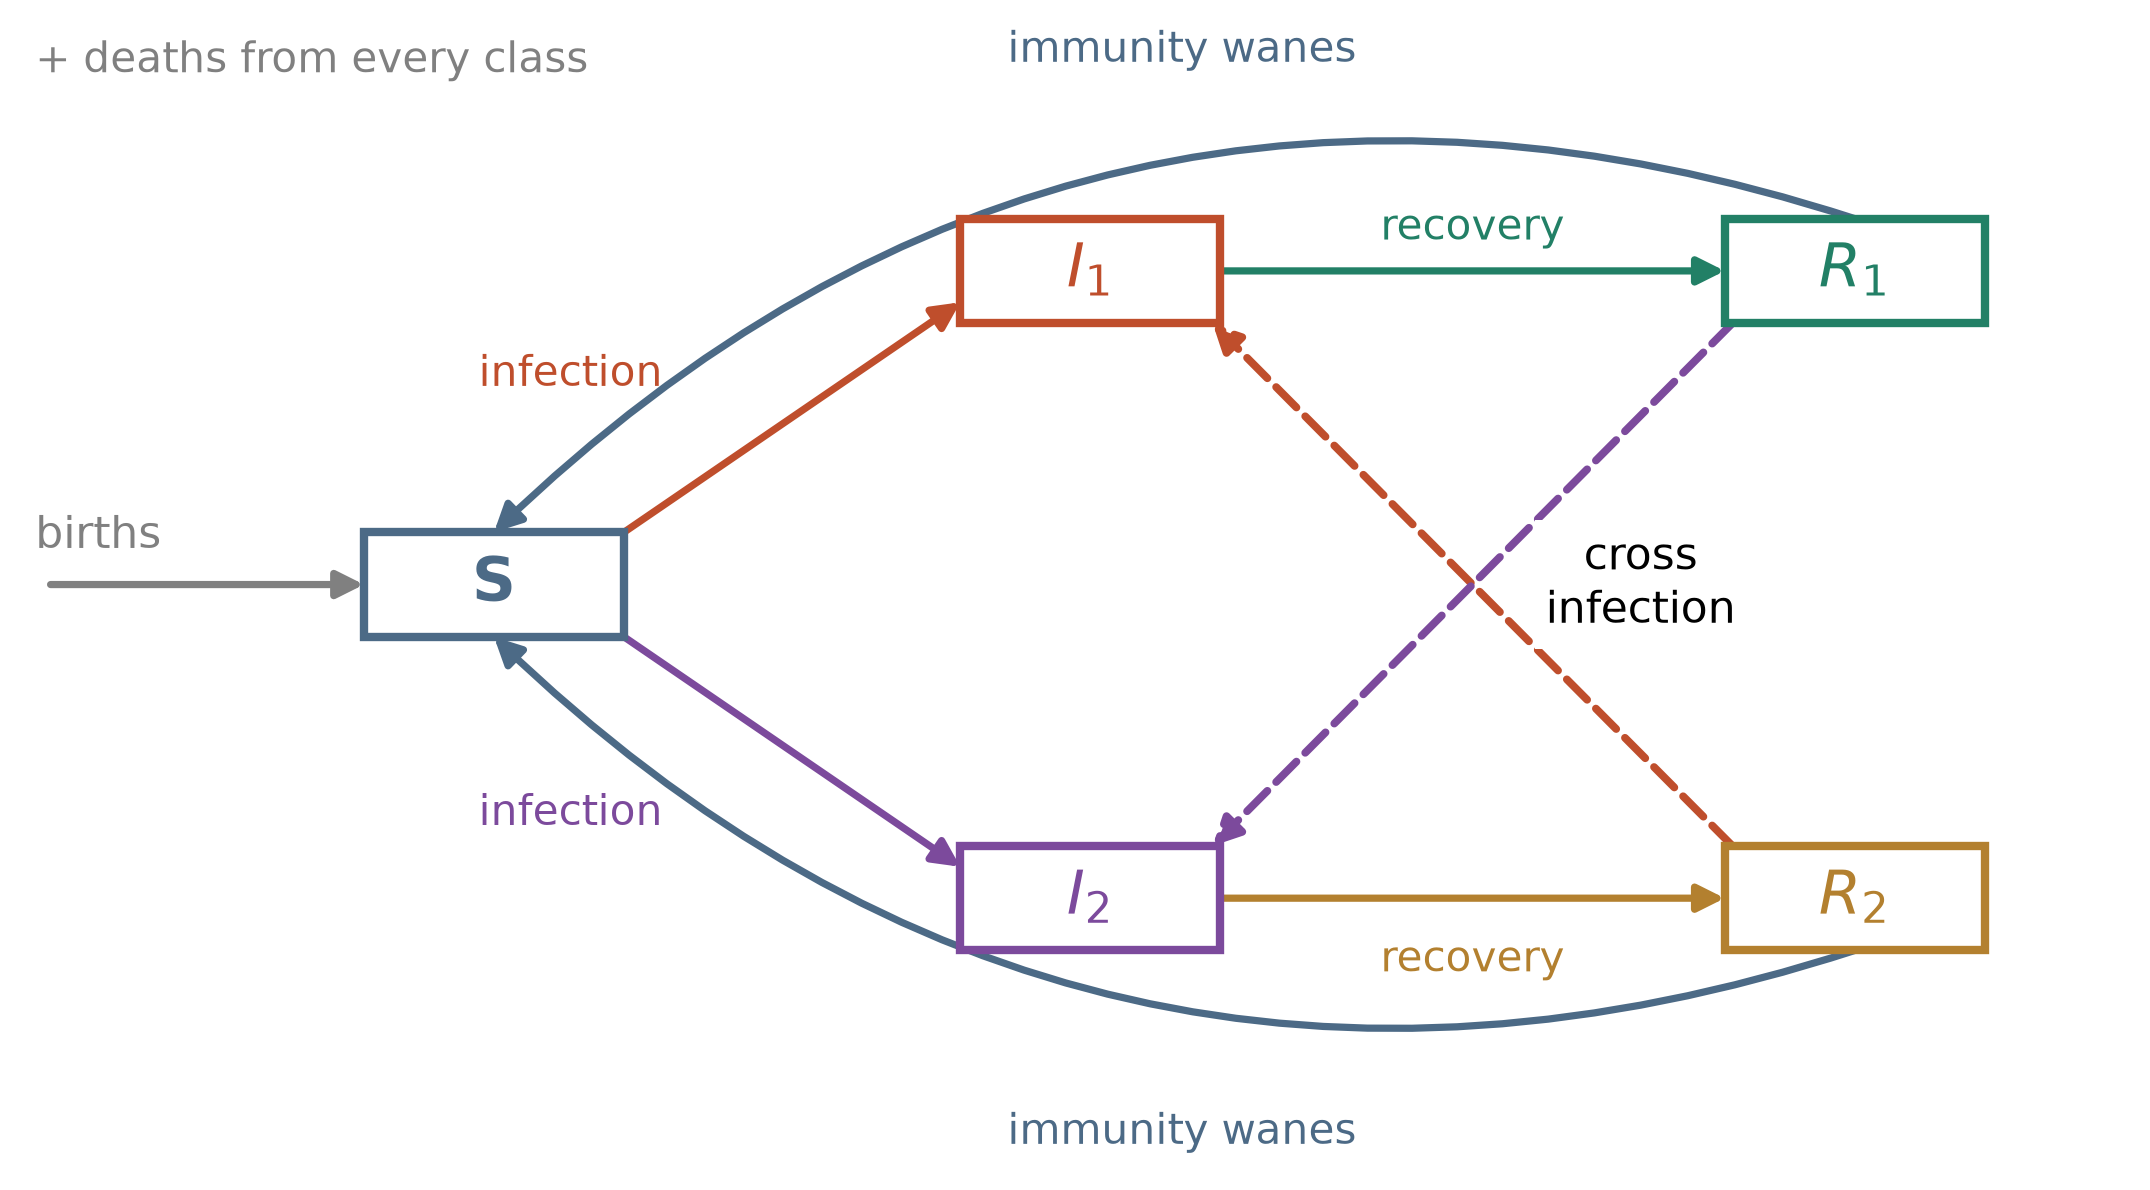
\includegraphics[width=0.70\textwidth]{img/slide_p2_cartoon.png}\\[0.2em]
\small
\hl{Cross infection} (dashed), as in the sheet's code: someone recovered from strain 2 can still catch strain 1, and the other way round.
Equations (2.1)--(2.5) as printed on the sheet have no dashed arrows: we test both.\\[0.5em]
\renewcommand{\arraystretch}{1.25}
\begin{tabular}{l c c c}
\rowcolor{aimsred}\color{white}& \color{white}infectious period & \color{white}immunity lasts & \color{white}$\mathcal R_0=\beta/(\gamma+\mu)$\\
Strain 1 & 1 week & 5 years & 2.31\\
\rowcolor{rowpink} Strain 2 & 2 weeks & 2 years & \textbf{3.84}\\
\end{tabular}
\end{frame}

% ---------------- 6. Part 2 coexistence ----------------
\begin{frame}{With 10,000 people, both models agree: the strains coexist}
\centering
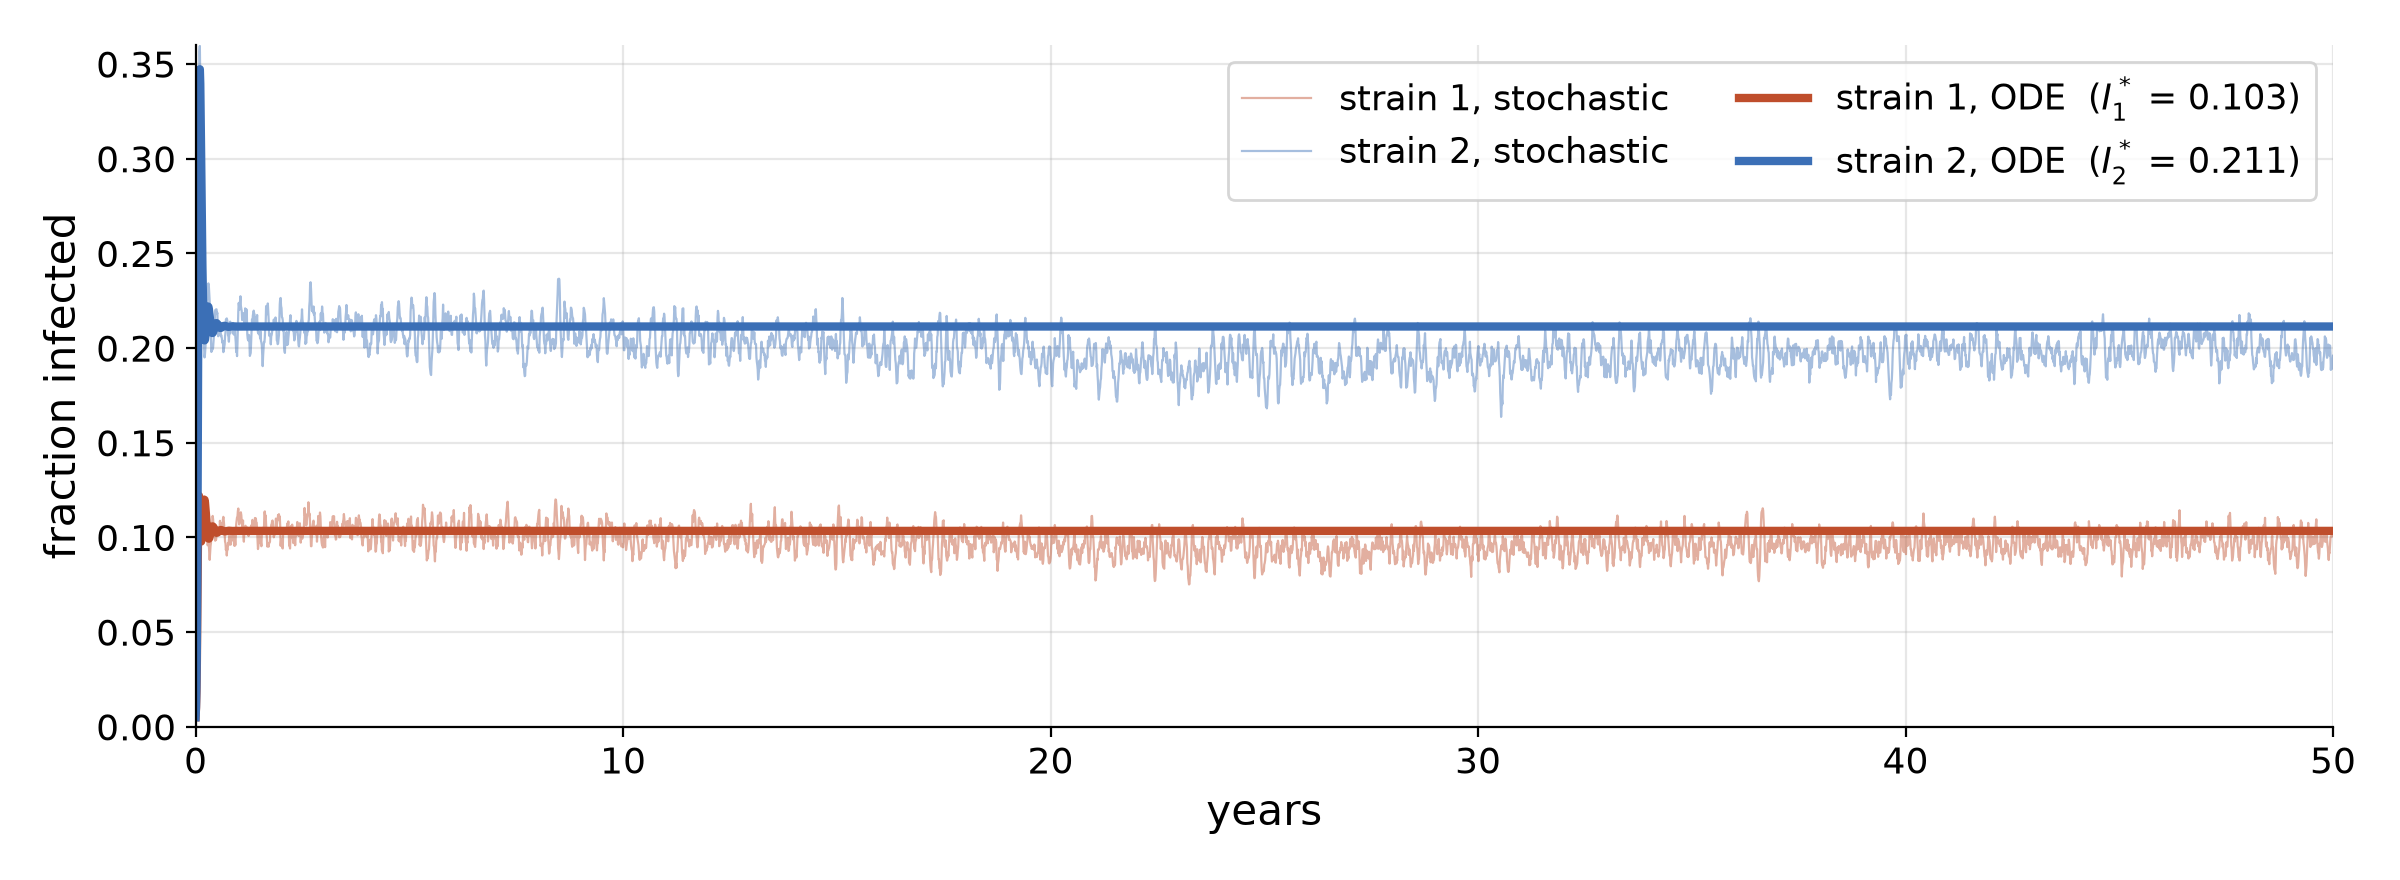
\includegraphics[width=0.94\textwidth]{img/slide_p2_coexistence.png}
\begin{itemize}\setlength\itemsep{0.4em}
  \item ODE: a \hl{stable coexistence}, reached after damped oscillations that fade within a year. No sustained cycles.
  \item Strain 2 has the larger $\mathcal R_0$ but does not win: each strain can invade the other (invasion numbers 3.83 and 2.27 $>1$), because people immune to one strain are still hosts for the other.
  \item The stochastic run stays close to the ODE, with no extinction in 50 years (slightly lower: random births and deaths took its population to about 9,830).
\end{itemize}
\end{frame}

% ---------------- 7b. Printed equations ----------------
\begin{frame}{Without cross infection, 10,000 people are not enough}
\centering
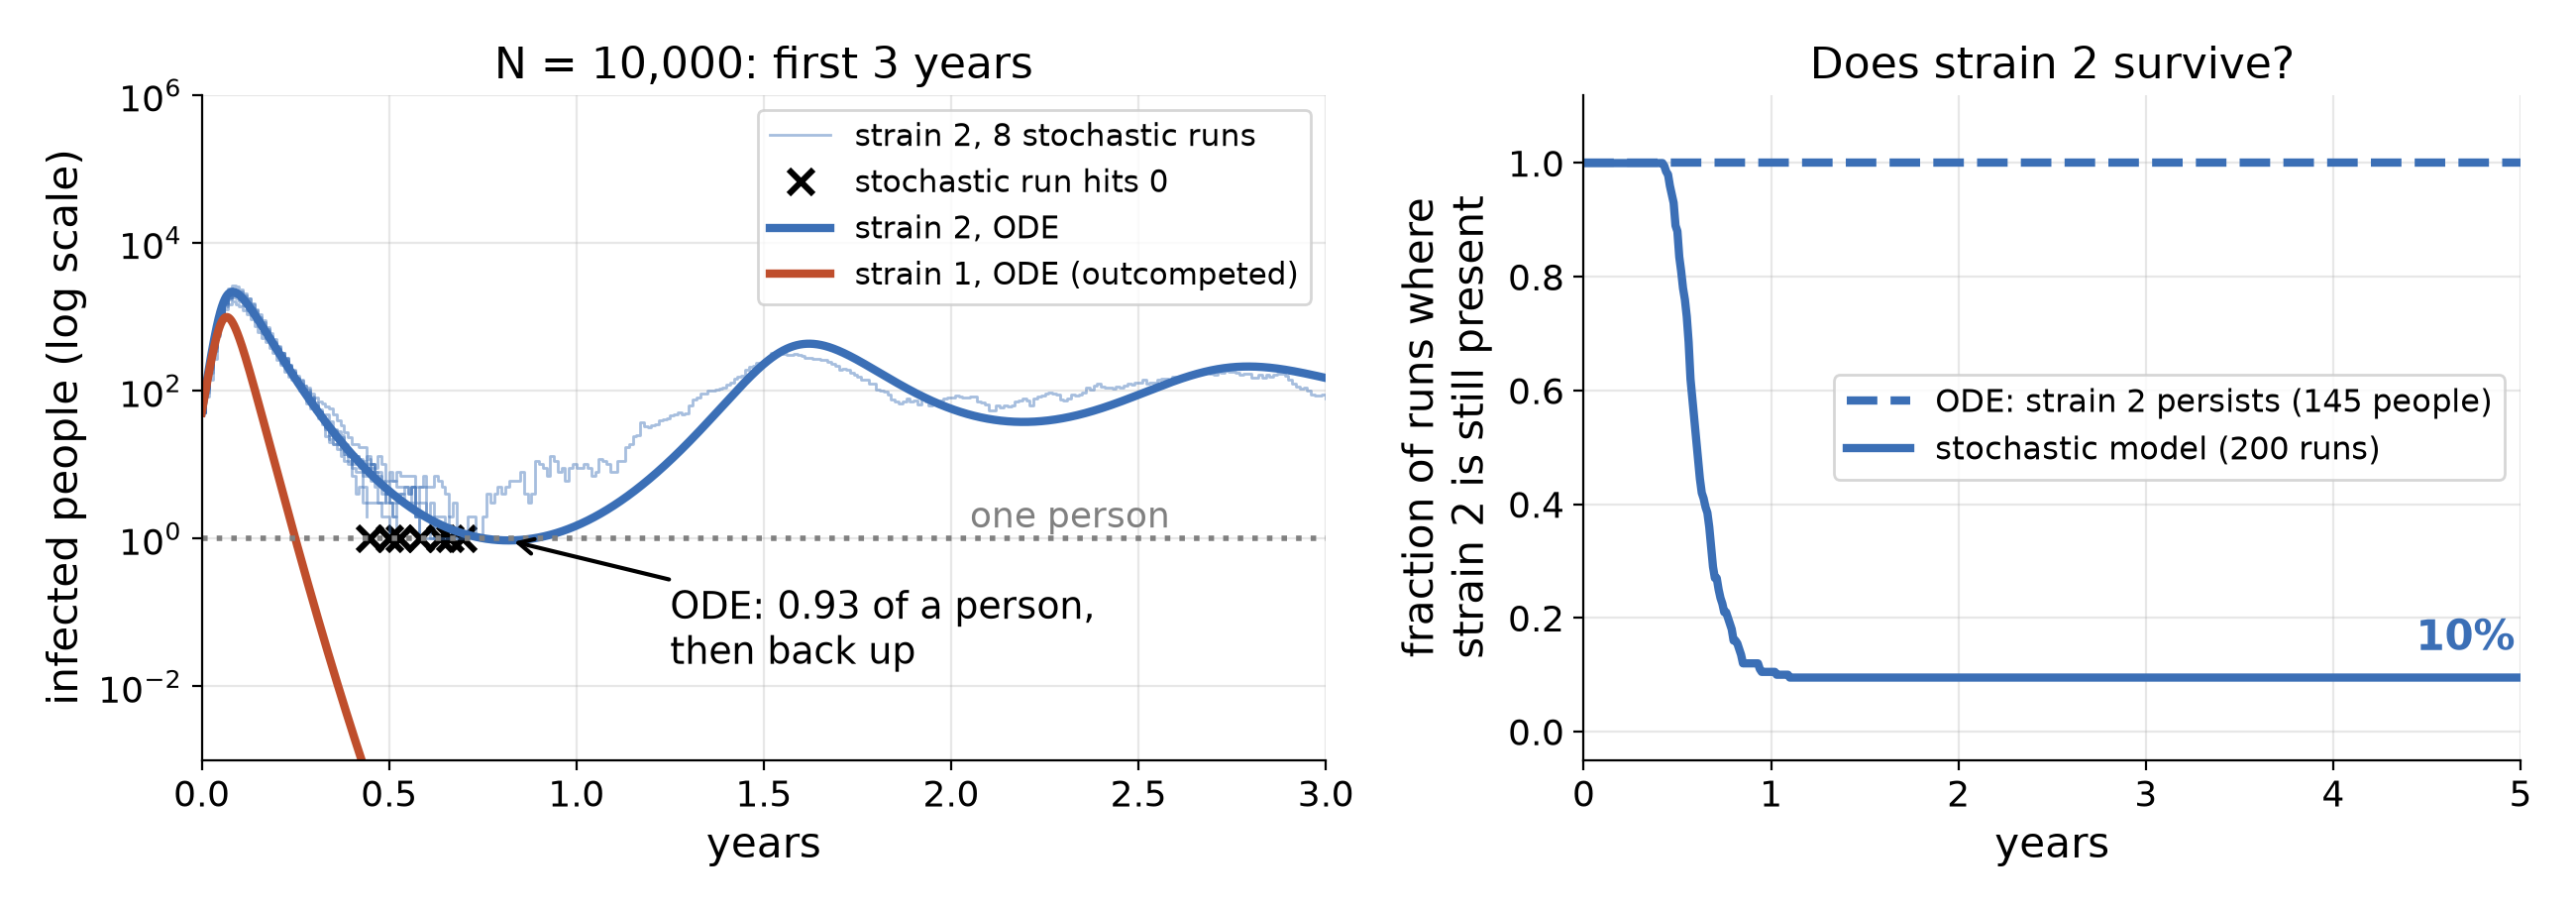
\includegraphics[width=\textwidth]{img/slide_p2_printed_equations.png}
\begin{itemize}\setlength\itemsep{0.4em}
  \item Equations (2.1)--(2.5) as printed: strain 2 ($\mathcal R_0=3.84$) outcompetes strain 1 ($\mathcal R_0=2.31$) in both models.
  \item \hl{ODE:} after its first peak, strain 2 falls to 0.93 of a person, then comes back and settles at 145 infected people. The disease survives.
  \item \hl{SSA:} a real outbreak cannot pass through 0.93 of a person. Strain 2 is still there after 5 years in only 19 of 200 runs (10\%): \hl{in most runs the disease disappears}.
\end{itemize}
\end{frame}

% ---------------- 7. Zero is final ----------------
\begin{frame}{Zero is final: a strain carried by few people can vanish for good}
\centering
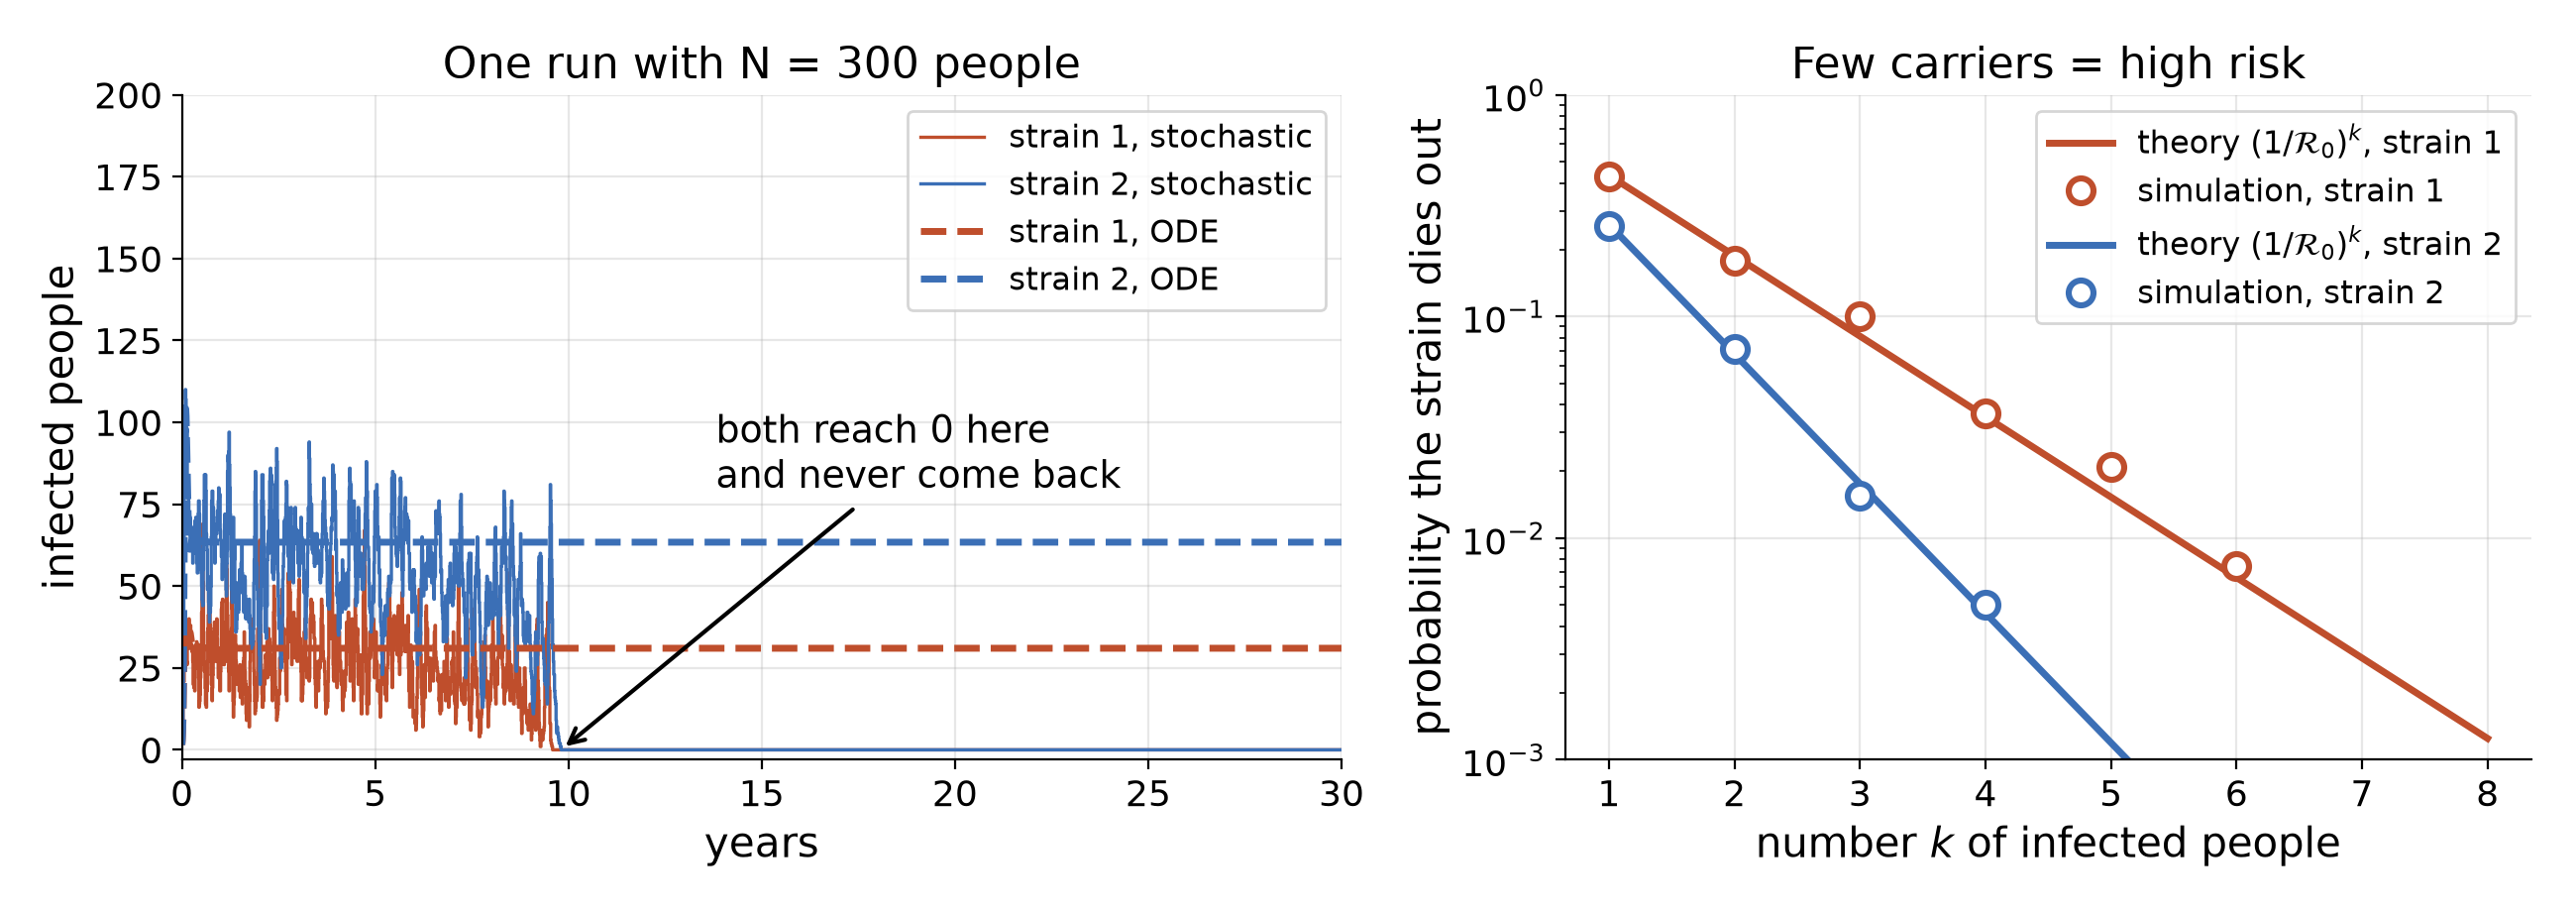
\includegraphics[width=\textwidth]{img/slide_p2_zero_is_final.png}
\begin{itemize}\setlength\itemsep{0.4em}
  \item \hl{ODE:} $I(t)=I(0)\,e^{\int_0^t g}>0$, so a strain can drop below one person and still rebound (0.93 of a person on the previous slide).
  \item \hl{SSA:} new infections need an infected person. At $I=0$ they stop, so a lost strain never returns.
  \item With $k$ infected people the risk of losing a strain is $(1/\mathcal R_0)^k$: 43\% for one case of strain 1.
\end{itemize}
\end{frame}

% ---------------- 8. Population size ----------------
\begin{frame}{Smaller populations lose strains that the ODE says persist}
\centering
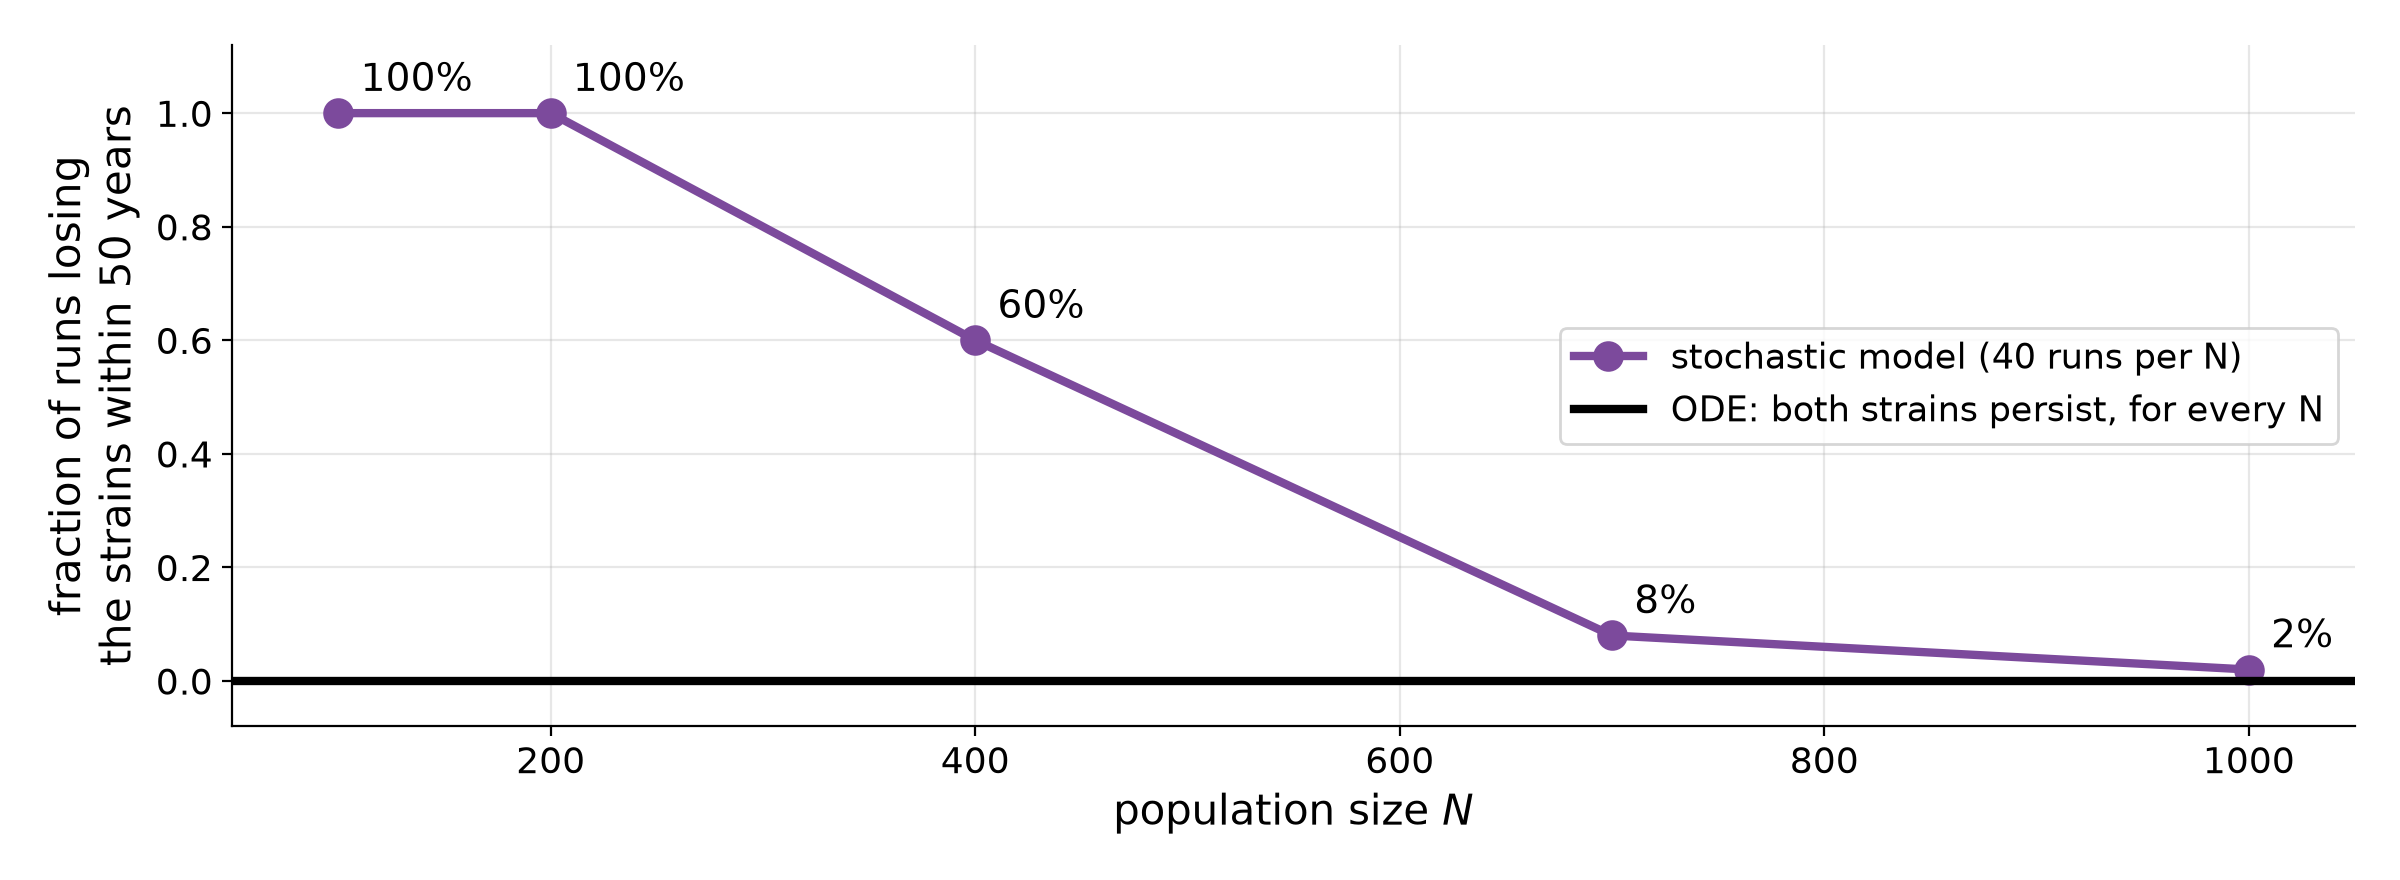
\includegraphics[width=\textwidth]{img/slide_p2_population_size.png}
\begin{itemize}\setlength\itemsep{0.4em}
  \item Same model, same parameters: only the population size changes. The ODE prediction does not depend on $N$.
  \item For $N\ge700$ all losses happen in the first year, when only 4 or 5 people carry each strain. At $N=10{,}000$: no loss in 50 years.
  \item The two strains are lost together: alone, each strain is sustained at a much lower level.
\end{itemize}
\end{frame}

% ---------------- 9a. Answer ----------------
\begin{frame}{So, does the disease survive?}
\centering
\renewcommand{\arraystretch}{1.45}\setlength{\tabcolsep}{4pt}
\small
\begin{tabular}{l l l l}
\rowcolor{aimsred}\color{white}Model & \color{white}People & \color{white}ODE (deterministic) & \color{white}SSA (stochastic)\\
One strain & $N=40$ & yes, 3.6 infected & \hl{no}: 0\% of runs\\
\rowcolor{rowpink} One strain & $N=100$ & yes, 12 infected & in 56\% of runs\\
Two strains, cross infection & $N=10{,}000$ & yes, both strains & yes, both (50 years)\\
\rowcolor{rowpink} Two strains, cross infection & $N=400$ & yes, both strains & lost in 60\% of runs\\
Two strains, cross infection & $N\le 200$ & yes, both strains & \hl{no}: lost in all runs\\
\rowcolor{rowpink} Two strains, as printed & $N=10{,}000$ & yes, strain 2 (145 infected) & \hl{mostly no}: 10\% of runs\\
\end{tabular}
\\[1.2em]
\normalsize
{\footnotesize Stochastic runs followed for 1 year (one strain), 50 years (cross infection) and 5 years (as printed).}\\[0.6em]
\callout{0.9\textwidth}{The ODE answers \hl{yes} in every row. The stochastic answer depends on \textbf{how many people carry the infection at its lowest point}.}
\end{frame}

% ---------------- 9. Take home ----------------
\begin{frame}{Take home: the ODE says what is possible, the SSA says what happens}
\begin{itemize}\setlength\itemsep{0.9em}
  \item \hl{Many carriers at all times:} the two models agree (endemic level, coexistence of the two strains with 10,000 people).
  \item \hl{Few carriers}, in a small population or after an outbreak crashes: chance removes infections and strains that the ODE keeps, and a lost strain does not return.
  \item \hl{Why it matters:} thresholds such as $N>\gamma/\beta$ or $\mathcal R_0>1$ are necessary for persistence, not sufficient. To know whether a disease or a strain survives in a real, finite community, we need the stochastic model.
\end{itemize}
\callout{0.9\textwidth}{Deterministic models describe the large population limit. Stochastic models tell us whether a disease actually survives.}
\end{frame}

\end{document}
